\documentclass[11pt]{beamer}
\usetheme{Madrid}

\usepackage[T1]{fontenc}
\usepackage[polish]{babel}
\usepackage[utf8]{inputenc}

\usepackage{amsmath}
\usepackage{amsfonts}
\usepackage{amssymb}
\usepackage{graphicx}

\DeclareMathOperator {\argmin}{argmin}

\graphicspath{images}

\author{Kamil Kowalski}

\title{Projekt SMiW}
% Informe o seu email de contato no comando a seguir
% Por exemplo, alcebiades.col@ufes.br
\newcommand{\email}{email}
%\setbeamercovered{transparent} 
\setbeamertemplate{navigation symbols}{} 
\institute[]{Politechnika Śląska\par Wydział Automatyki Elektroniki  i Informatyki} 
\date{\today} 

\bibliographystyle{apalike}

\begin{document}

\begin{frame}
\titlepage
\end{frame}

\section{Opis założeń}

\begin{frame}{Problem do rozwiązania}

    \begin{itemize}
        \item Brak ostrzeżeń o niskim poziomie paliwa
        \item Alarm uruchamia się po kilku próbach rozpalenia -- zwiększone zużycie elementu grzewczego
    \end{itemize}

\end{frame}

\begin{frame}{Opis działania}
    
    \begin{itemize}
        \item Podgląd stanu zasobnika w aplikacji na telefony stacjonarne
        \item Alerty o niskim poziomie paliwa (powiadomienie na telefon)
        \item Wyświetlanie bieżącej ilości paliwa na ekranie LCD
    \end{itemize}

\end{frame}

\section{Opis systemu}

\begin{frame}{Czujnik odległości}
 Wybrany czujnik: VL53L0X.
 \begin{figure}
     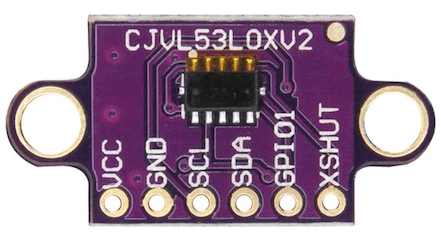
\includegraphics[width=0.2\textwidth, angle=-90]{images/vl53l0x}
 \end{figure}
 \begin{itemize}
     \item Zasięg: 0.03m - 2.0m
     \item Zakres napięć: 2.6V - 5.5V
     \item Interface: I2C
 \end{itemize}

\end{frame}

\begin{frame}{Wyświetlacz LCD}
        Wybrany wyświetlacz: LCM1602 z ekspanderem IO.
        \begin{itemize}
            \item Napięcie zasilania: 5V
            \item Interface: I2C
        \end{itemize}

        \begin{figure}
            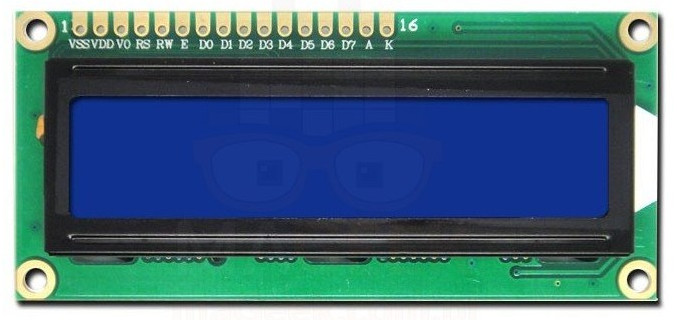
\includegraphics[width=0.3\textwidth]{images/LCM1602}
            \caption{Wyświetlacz LCM1602}
        \end{figure}

        \begin{figure}
            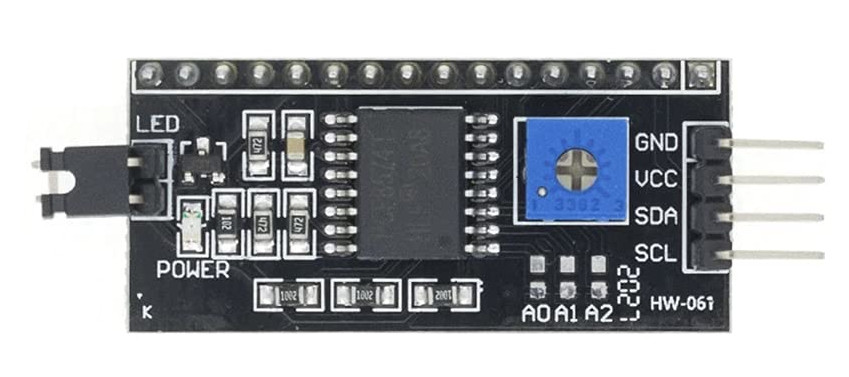
\includegraphics[width=0.3\textwidth]{images/HW-061}
            \caption{Ekspander portów HW-061}
        \end{figure}

\end{frame}

\begin{frame}{Mikrokontroler}
    Wybrany mikrokontroler: ESP32 DevKit v1.
    \begin{figure}
        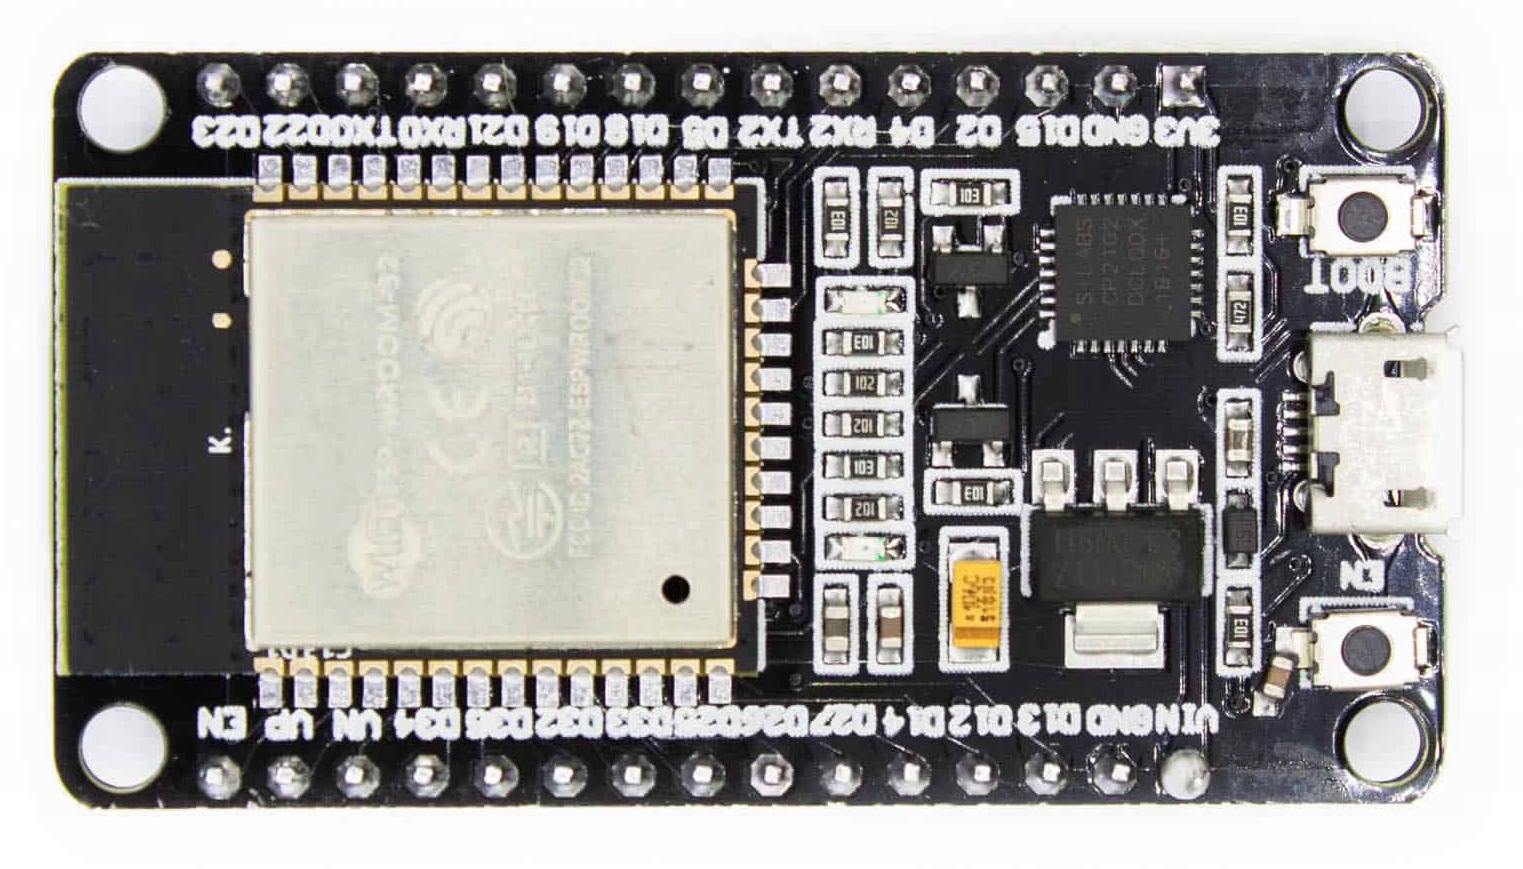
\includegraphics[width=0.5\textwidth]{images/ESP32}
    \end{figure}
    
    \begin{itemize}
        \item Łączność WiFi
        \item Napięcie zasilania: 5V
        \item Obsługa I2C
    \end{itemize}
\end{frame}

\begin{frame}{Inne części}
    \begin{itemize}
        \item Układ będzie składał się z części modułu oraz części głównej, zostaną one połączone kablem micro USB - micro USB
        \item Zasilanie dostarczone będzie przez 5V ładowarkę micro USB 
    \end{itemize}
\end{frame}

\begin{frame}{Schemat}

    \begin{figure}
        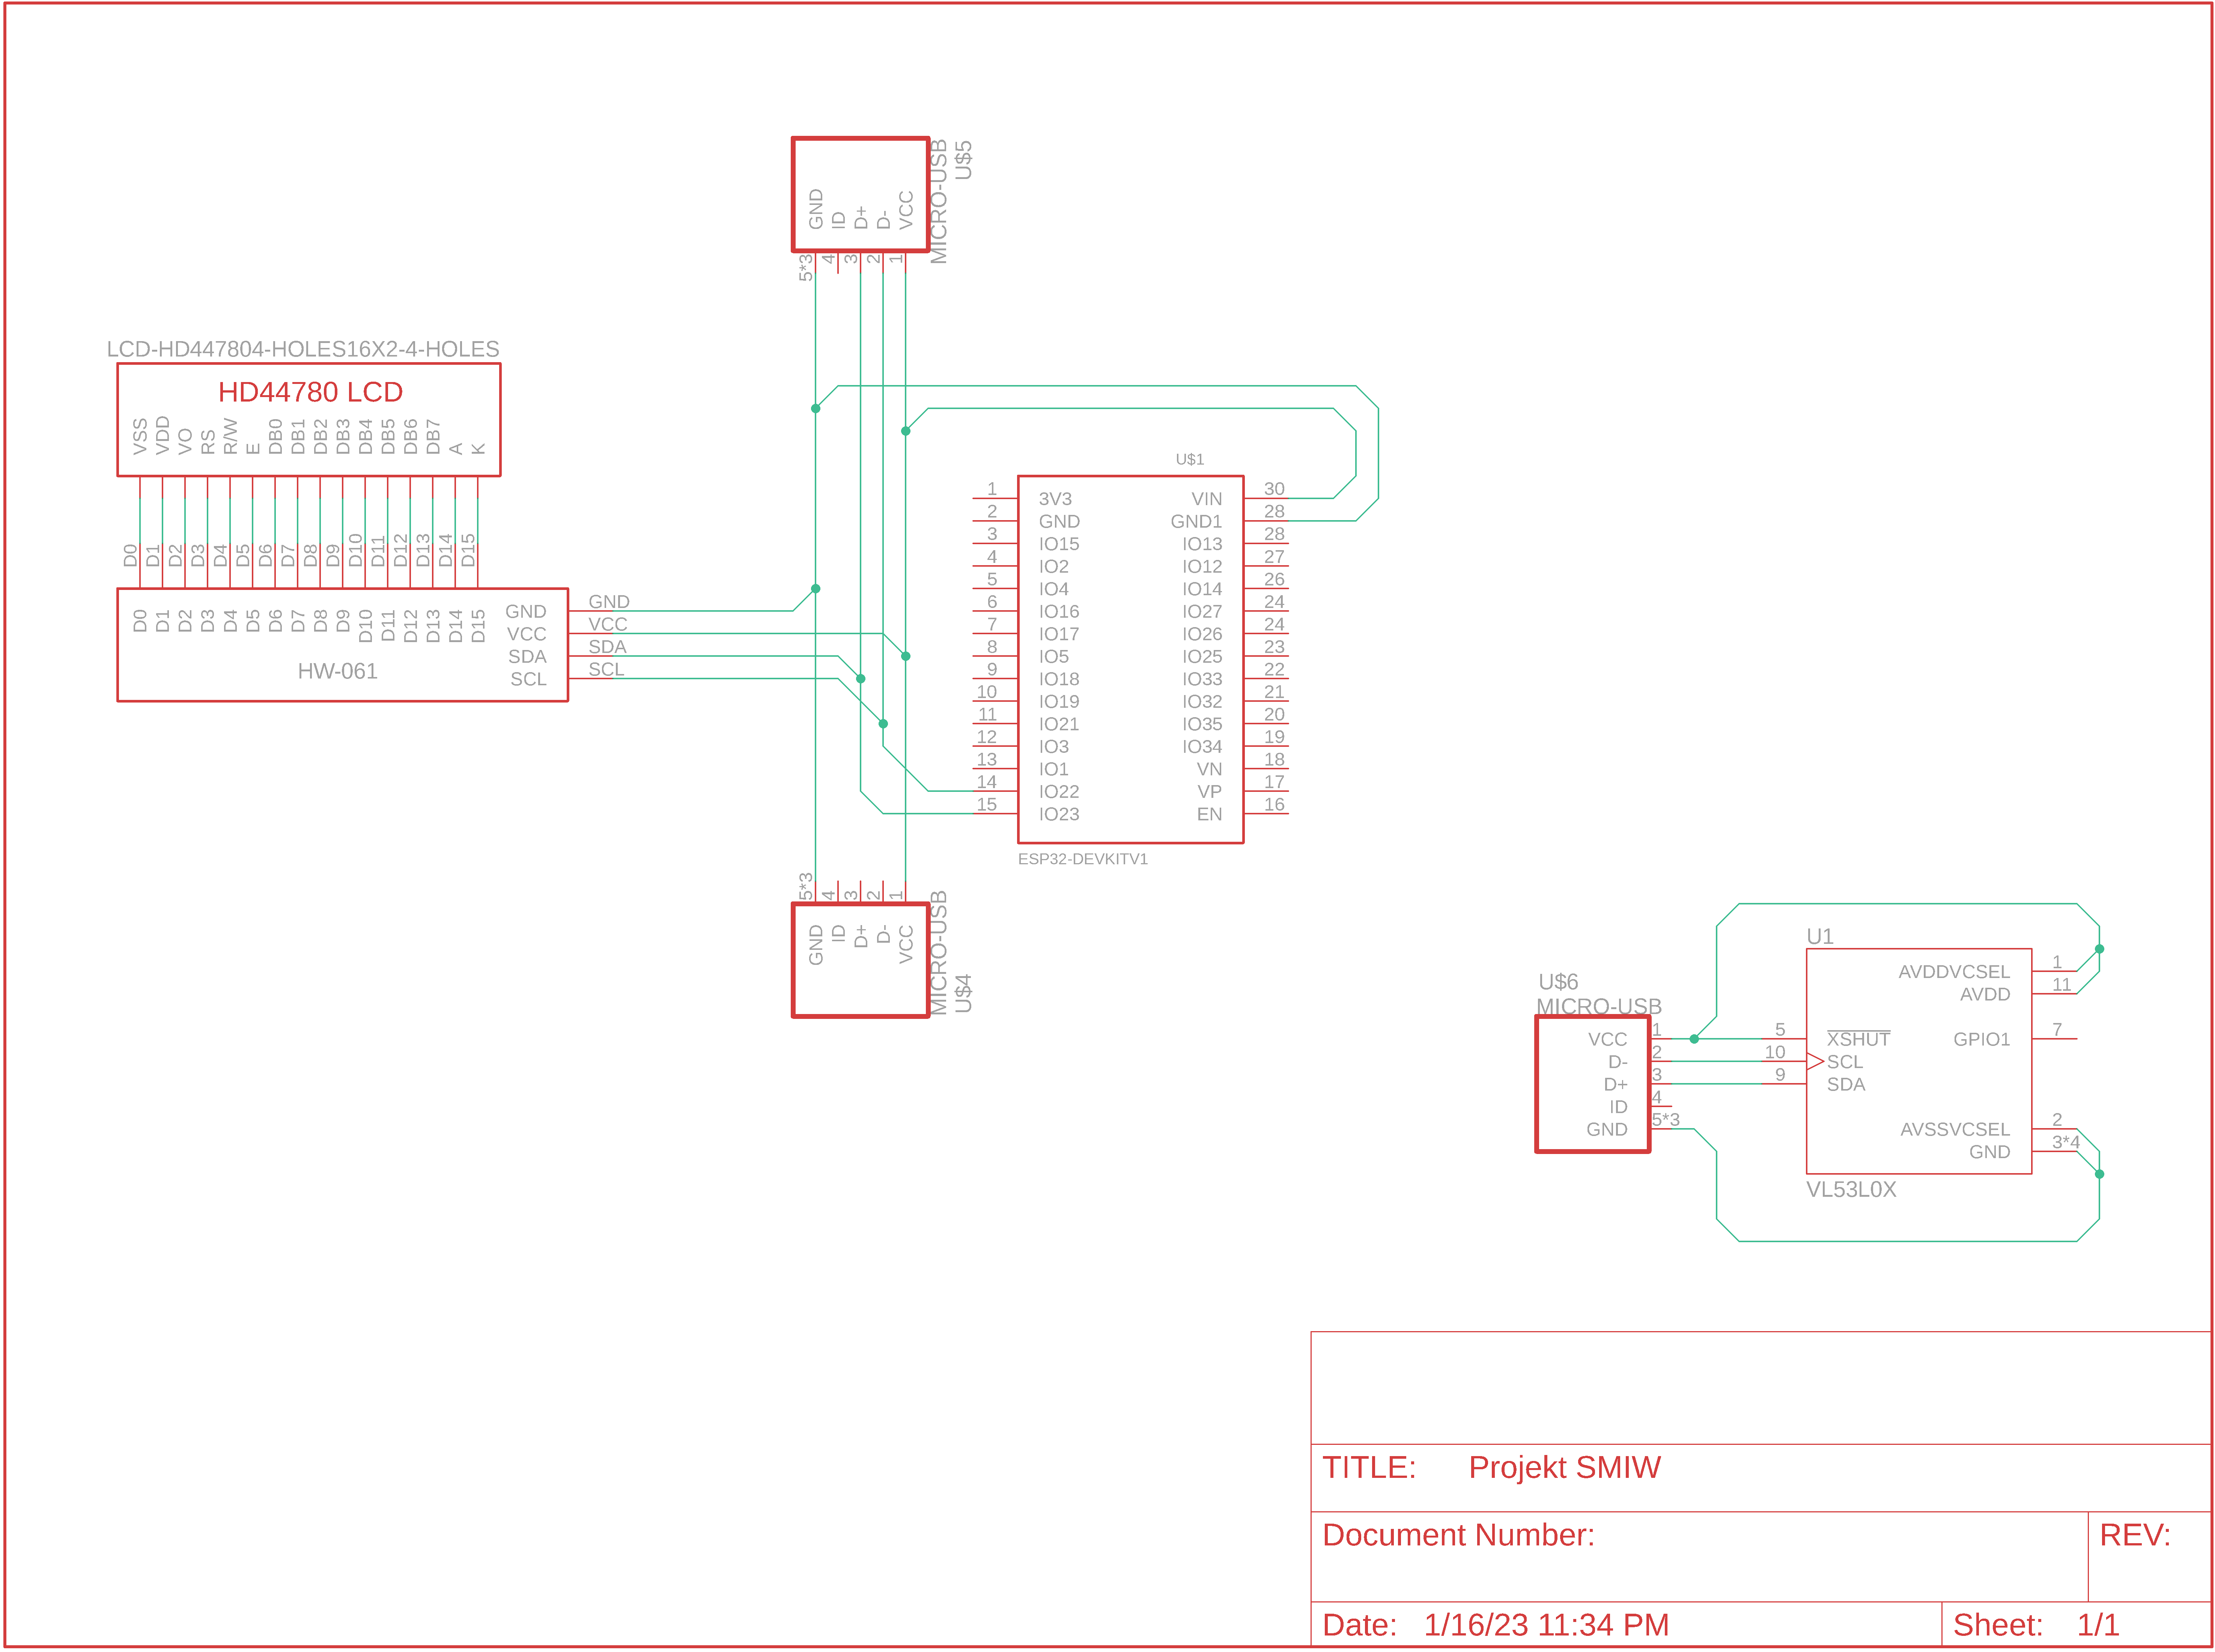
\includegraphics[width=0.8\textwidth]{images/schematic}
    \end{figure}
\end{frame}

\end{document}
